\section{Einleitung in die Thesis} \label{Einleitung in die Thesis}
	
\newpage
\section{Auftragsinterpretation} \label{Auftragsinterpretation}

	\textbf{Problembeschreibung:} \vspace{2mm} 
	\\
	Roboter finden in der Industrie eine immer breiter werdende Anwendung und sind aus vielen Prozessen
	nicht mehr wegzudenken. Ein grosser Beschaffungs- und Inbetriebnahmeaufwand machen es jedoch
	für viele Unternehmen schwierig, ein Roboter in ihre Prozesse zu integrieren. Dadurch werden
	zeitintensive und monotone Arbeiten oftmals noch manuell von Mitarbeitern durchgeführt. Eine grosse
	Hürde des Robotersystems ist der konventionelle Robotersoftwareansatz, welcher ein Grundverständnis
	für die Programmierung des Roboters voraussetzt. Für Veränderungen im Prozessablauf wird dadurch
	zwingend ein Programmierer benötigt.
	\vspace{3mm}
	
	\textbf{Beschreibung des Auftrages:} \vspace{2mm} 
	\\
	Die Thesis beschäftigt sich mit der Frage, wie ein Roboter einfacher und standardisiert programmiert
	werden kann. Hierfür wird der Ansatz einer Rezeptursteuerung (bekannt aus Pharmaprozessen)
	analysiert. Dabei wird untersucht, ob ein solcher Ansatz für Roboteranwendungen geeignet ist und wie
	dieser eingesetzt werden kann. Ein zentrales Element ist dabei der skill-basierte Aufbau eines
	Roboterprogramms.
	\\
	\linebreak
	Die konkreten Ziele der Thesis sind wie folgt definiert:
	\begin{itemize}
		\item Analyse des Ansatzes einer Rezeptursteuerung für Roboteranwendungen
		\item Analyse und Definierung von geeigneten Skills
		\item Softwaremässige Umsetzung des skill-basierten Ansatzes
		\item Die Software soll auf Fehler bei der Prozessdurchführung des Roboters reagieren können
	\end{itemize}
	\addvspace{5mm}
	
	\textbf{Auftragskontext:} \vspace{2mm} 
	\\
	Die Thesis findet als BFH-internes Projekt statt, welches aus dem Forschungsprojekt «ARCOBA»
	entstanden ist. Das Ziel dieses Forschungsprojektes ist die Entwicklung und Demonstration neuartiger
	Konzepte für Roboterplattformen bezüglich agiler Fertigung.
	\vspace{3mm}
	
	\textbf{Abgrenzungen:} \vspace{2mm} 
	\\
	Die Thesis beschäftigt sich nicht mit der Umsetzung einer konkreten industriellen Anwendung. Es ist
	jedoch möglich, dass Erkenntnisse aus dieser Thesis für zukünftige Automatisierungsprojekte
	verwendet werden.
	\vspace{3mm}
	
	\textbf{Projektorganisation:} \vspace{0mm} 
	
	\begin{table}[ht]
		\centering
		\colorlet{BFH-table}{BFH-MediumBlue!10}
		\colorlet{BFH-tablehead}{BFH-MediumBlue!50}
		\begin{bfhTabular}{llll}
			Rolle		& 	Wer							&	Status			&	Kontakt		\\\hline
			
			Advisor		 & Prof. Melchior Borer			& Dozent BFH 		& 	\href{mailto:melchior.borer@bfh.ch}{melchior.borer@bfh.ch}  	\\\hline
			Experte		 & Prof. Dr. Norman Urs Baier	& Dozent BFH		&	\href{mailto:norman.baier@bfh.ch}{norman.baier@bfh.ch}		\\\hline
			Student		 & Yannick Spatz 				& Master-Student	&	\href{mailto:yannick.spatz@bfh.ch}{yannick.spatz@bfh.ch}	\\\hline
			
		\end{bfhTabular}
		
		\captionsetup{justification=centering}
		\caption{Projektorganisation}
		\label{Projektorganisation}
	\end{table}
	

\section{Zeitplan der Thesis} \label{Zeitplan der Thesis}

	Der erstellte Zeitplan dient als erste grobe Orientierung und stellt eine vorläufige Einschätzung des Projektverlaufs dar. Da der genaue Umfang der Aufgabenstellung für diese Thesis nur schwer im Voraus vollständig abzuschätzen ist, kann der Projektrahmen entsprechend variieren. Insbesondere die Entwicklung der Software ist ein dynamischer und iterativer Prozess.
	\\
	Daher ist der Zeitplan als flexibles Arbeitstool zu verstehen, das zwar eine klare zeitliche Struktur vorgibt, sich jedoch im Laufe des Projekts an veränderte Anforderungen und Erkenntnisse anpassen kann. Er soll einerseits helfen, die einzelnen Meilensteine im Blick zu behalten, und andererseits als Leitfaden dienen, um trotz aufkommender Änderungen einen festen Rahmen für den Projektfortschritt zu gewährleisten. Die kontinuierliche Überprüfung und gegebenenfalls Anpassung des Zeitplans ist ein integraler Bestandteil dieses Prozesses, um sicherzustellen, dass das Projekt im vorgesehenen zeitlichen Rahmen bleibt. 

	\begin{figure}[h!]
		\centering
		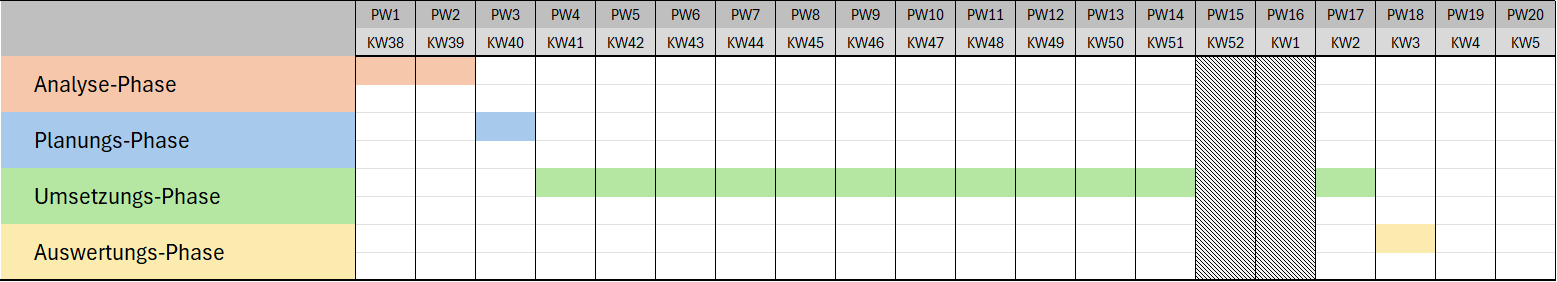
\includegraphics[width=1\textwidth]{01_Rahmen_der_Arbeit/Terminplanung_V2}
		\caption{Grobzeitplan der Thesis}
		\label{fig:Grobzeitplan}
	\end{figure}
	
	\begin{bfhNoteBox}
		Eine detaillierte Version des endgültigen Zeitplans wird im Anhang aufgeführt 
	\end{bfhNoteBox} 

		